\documentclass{article}
\usepackage{graphicx}

\title{Lab 2 Report}
\author{Muhammad Shafeen\\ Roll No: 22P-9278\\ Bachelor of Artificial Intelligence}
\date{\today}

\begin{document}

\maketitle

\section{Introduction}
This document provides an explanation of the `ls` command in Linux, which is used to list directory contents. The `ls` command can be used with various options to display the contents in different formats.

\section{Commands and Outputs}
\subsection{Command: \texttt{ls -a}}
The `ls -a` command lists all the files and directories in the current directory, including hidden files (those starting with a dot `.`). Below is the output of the `ls -a` command:
\begin{center}
    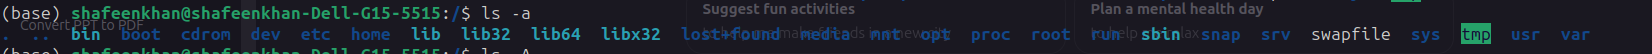
\includegraphics[width=\linewidth]{1.png}
\end{center}

\subsection{Command: \texttt{ls -A}}
The `ls -A` command is similar to `ls -a`, but it does not list the `.` (current directory) and `..` (parent directory) entries. Below is the output of the `ls -A` command:
\begin{center}
    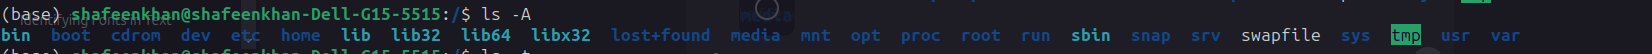
\includegraphics[width=\linewidth]{2.png}
\end{center}

\subsection{Command: \texttt{ls -t}}
The `ls -t` command lists files and directories sorted by modification time, with the most recently modified files listed first. Below is the output of the `ls -t` command:
\begin{center}
    
\includegraphics[width=\linewidth]{3.png}
\end{center}

\subsection{Command: \texttt{pwd}}
The `pwd` (print working directory) command displays the full path of the current working directory. This is particularly useful to know where you are within the file system. Below is the output of the `pwd` command:
\begin{center}
    
\includegraphics[width=0.8\linewidth]{4.png}
\end{center}



\subsection{Command: \texttt{adduser}}
The `adduser` command is used to add a new user to the system. The image below shows an attempt to add a new user named `shafeencopy`. Initially, the command was entered incorrectly as `adduser`, which requires a single username argument. After correcting the command to `adduser shafeencopy`, a new user was successfully added, and the system prompted for additional information such as the full name, room number, and phone numbers. Below is the output of the `adduser` command:
\begin{center}
    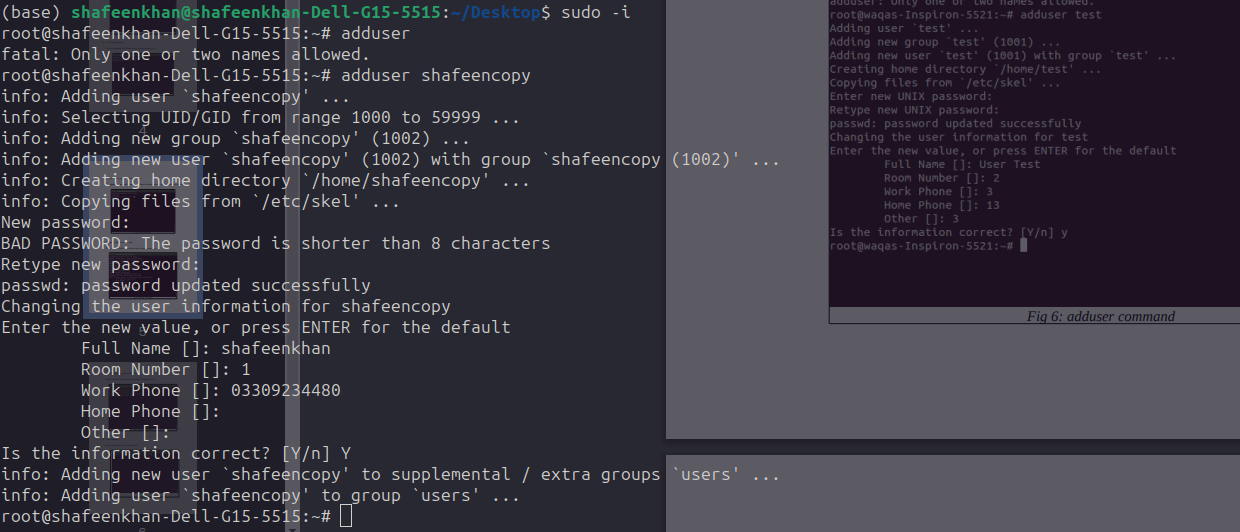
\includegraphics[width=0.8\linewidth]{5.png}
\end{center}

\subsection{Command: \texttt{Sudo}}
After using `sudo`, the package installation proceeded. Below is the output of the `apt install tree` command:sudo apt install tree 
sudo gives root privileges and allows installation for some sensitive directories
\begin{center}
    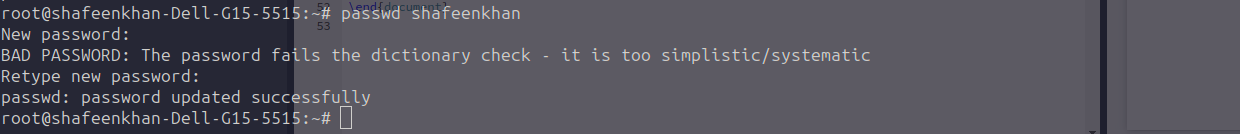
\includegraphics[width=0.8\linewidth]{6.png}
\end{center}


\subsection{Command: \texttt{passwd}}
The `passwd` command is used to change a user's password. In this case, the password for the user `shafeenkhan` was being updated. Initially, the password entered was too simplistic, triggering a warning that it failed the dictionary check. However, after re-entering the password, it was updated successfully. Below is the output of the `passwd` command:
\begin{center}
    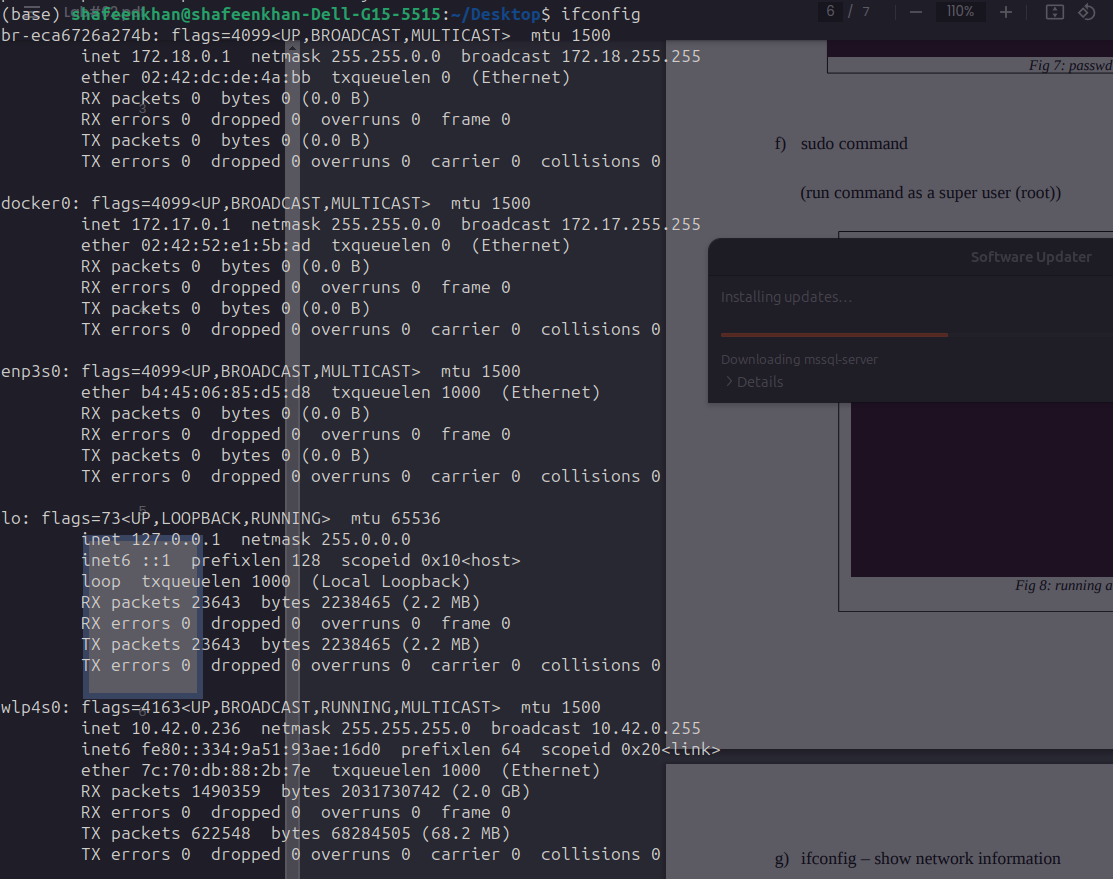
\includegraphics[width=0.8\linewidth]{7.png}
\end{center}

\subsection{Command: \texttt{ifconfig}}
The `ifconfig` command is used to configure and display the network interfaces in a Unix-like operating system. In this example, the command provides detailed information about various network interfaces on the system, including `br-eca6762a74b`, `docker0`, `enp3s0`, `lo`, and `wlp4s0`. Each interface shows details like IP addresses, netmask, broadcast address, and statistics for transmitted and received packets. Below is the output of the `ifconfig` command:
\begin{center}
    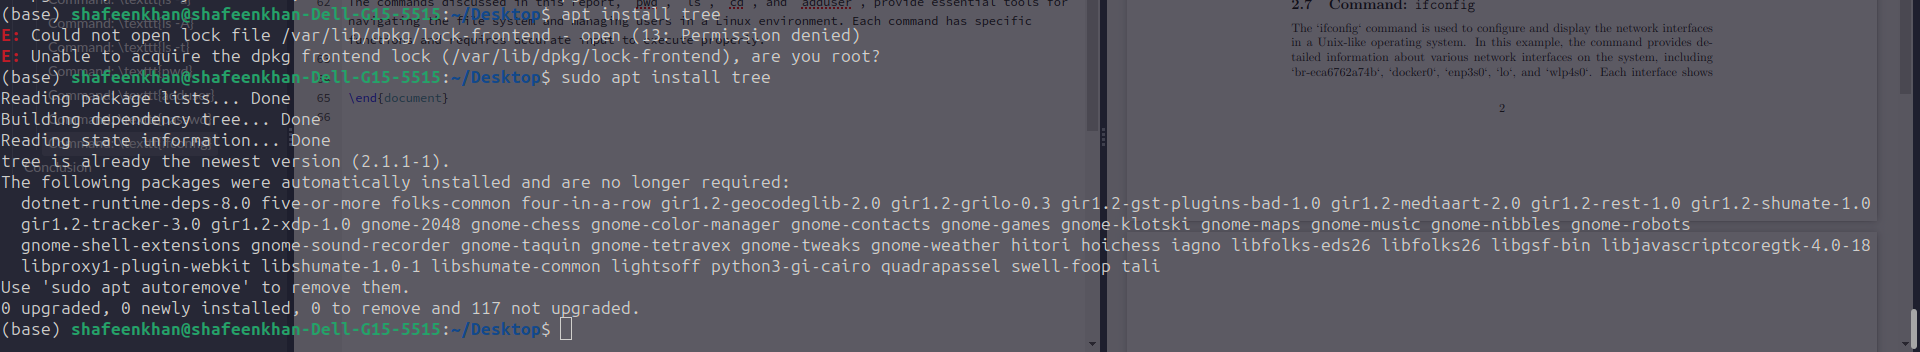
\includegraphics[width=0.8\linewidth]{8.png}
\end{center}

\subsection{Command: \texttt{iwconfig}}
The `iwconfig` command is used to configure wireless network interfaces in Linux. It provides detailed information about wireless connections, including the ESSID, frequency, signal quality, and various other statistics. In the example below, the command displays information for the wireless interface `wlp4s0`, while other interfaces like `lo`, `enp3s0`, `br-eca6762a74b`, and `docker0` report no wireless extensions. Below is the output of the `iwconfig` command:
\begin{center}
    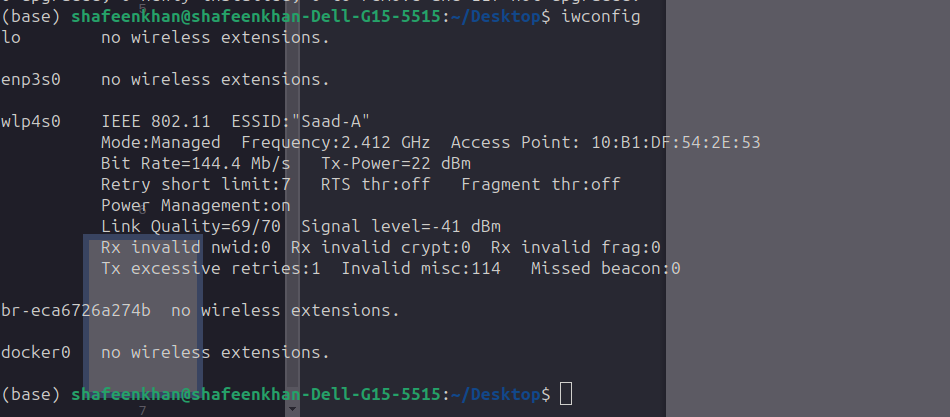
\includegraphics[width=0.8\linewidth]{9.png}
\end{center}


\section{Conclusion}
In this lab, we explored various essential Linux commands used for system navigation, user management, network configuration, and software installation. Commands like `pwd` and `ls` help in understanding and navigating the file system, while `cd` allows for directory changes. The `adduser` and `passwd` commands are crucial for managing users on the system. Networking tools such as `ifconfig` and `iwconfig` provide detailed insights into the network interfaces and wireless configurations. Lastly, the `apt install` command is vital for package management in Debian-based distributions. Understanding these commands and their outputs is fundamental for effective system administration and troubleshooting in a Linux environment.



\end{document}
